%%
%%
\documentclass[12pt]{book}
\usepackage{amsfonts}
\usepackage[fleqn]{amsmath}
\usepackage{amssymb}
\usepackage[fleqn]{mathtools}
\usepackage{graphicx}
\usepackage{hyperref}
\usepackage{tikz}
\usepackage{siunitx}
\usepackage{float}
\setlength{\textheight}{10in}
\setlength{\textwidth}{7.4in}
\setlength{\topmargin}{-0.75in}
\setlength{\oddsidemargin}{-0.5in}
\setlength{\evensidemargin}{-0.5in}
\setlength{\parskip}{0.15in}
\setlength{\parindent}{0in}

\begin{document}


\vspace{-1.0in}\begin{center}
\Large{MHF4UR : Pre-AP Advanced Functions }

\Large{Assignment \#1}


\end{center}

%\medskip

\vspace{0.015in}\hrulefill\ 

\textbf{Reference Declaration} %  Fill in your Reference Declarations in this section before your submit your assignment.

Complete the Reference Declaration section below in order for your assignment to be graded.

If you used any references beyond the course text and lectures (such as other texts, discussions with colleagues or online resources), indicate this information in the space below.  If you did not use any aids, state this in the space provided. 

Be sure to cite appropriate theorems throughout your work. You may use shorthand for well-known theorems like the FT (Factor Theorem), RRT (Rational Root Theorem), etc. 

Note: Your submitted work must be \textbf{your original work}. 

Family Name: Do \\%Family Name Here
First Name: Kien %First Name Here

Declared References: Help from my dad and discussed with Isaac about question $1d$. 

% Type your references here.
% You can use as many lines as required.

\vspace{0.015in}\hrulefill\ 

\newpage

%%%%%%%%%%%% PROBLEMS START HERE

\begin{enumerate}

%% PROBLEM 1
\item A set $A$ is said to be \emph{closed} or to have \emph{closure} under a given operation $\Delta$ if when $a,b \in A$ we also have $a \Delta b \in A$. 

\begin{enumerate}
%% 1a
\item Prove that the even integers are closed under addition.\\

\textbf{Solution:}

An even integer is an integer that can be divided by 2 without having any remainders. Therefore, even integers can be represented as $2x$ where $x$ is any integer.\\

Let the sum of two even integers be $m$, $x$ and $y$ be any integer. We have:\\
$m = 2x + 2y$\\
$m = 2(x+y)$\\
$\dfrac{m}{2} = x + y$\\

We can see that no matter what $m$ equals, $\dfrac{m}{2}$ will always equal an integer, $x + y$, as integers are closed under addition. Since $\dfrac{m}{2}$ always equals an integer without having any remainders, $m$ is an even integer.\\

\textbf{Therefore, even integers are closed under addition.\\}
%% 1b
\item Prove that the odd integers are closed under multiplication.\\

\textbf{Solution:}

An odd integer can be defined and mathematically represented as \textit{an even number + 1}. We will take a look at this statement again as the proof progresses.\\

Let $a$ and $b$ be two even integers, and $x$ be the product of two odd integers. The multiplication of two odd integers can be represented as follows:
\setcounter{equation}{0}
\begin{align}
    x &= (a + 1) \times (b + 1)\\
    x &= ab + a + b + 1
\end{align}
Let's take a look at line (2) of the equation above. Since even integers are closed under addition and $a$ and $b$ are integers, the product of $ab$ is also an integer. This is because $ab$ just means 
$\overbrace{a + a + a... }^\text{b}$. Following the same rule, the sum of $a + b$ is also an even integer. This means that $ab + a + b$ can be entirely represented as some number c, where c is an even integer.\\
To simply the equation above, we have
\setcounter{equation}{0}
\begin{align}
    x &= (a + 1) \times (b + 1)\\
    x &= ab + a + b + 1\\
    x &= c + 1
\end{align}
Since the definition of an odd integer is \textit{an even integer + 1} and c is an even integer, $x$ is an odd integer.\\

\textbf{Therefore, odd integers are closed under multiplication.}

%% 1c
\item Prove that odd functions are closed under subtraction.\\

\textbf{Solution:}

An odd function is a function where $f(x) = -f(-x)$ or $-f(x) = -f(-x)$. Consider two odd functions $f(x)$ and $g(x)$ and the difference of $f(x)$ and $g(x)$ be $h(x)$. Prove that $h(x) = -h(-x)$.\\

We know that:
\setcounter{equation}{0}
\begin{align}
    h(x) &= f(x) - g(x)\\
    h(x) &= -f(-x) - [-g(-x)]\\
    h(x) &= -f(-x) + g(-x)
\end{align}
Modify the equation on line (1). First, multiply $x$ on both sides by -1 then multiply both sides of the equation by -1.
\begin{align}
    h(x) &= f(x) - g(x)\\
    h(-x) &= f(-x) - g(-x)\\
    -h(-x) &= -f(-x) + g(-x)
\end{align}
Since $h(x) = -f(-x) + g(-x)$ on line (3) and $-h(-x) = -f(-x) + g(-x)$ on line (6), we can conclude that $h(x) = -h(-x)$ from using the logic of $a = b$ and $b = c$, therefore $a = c$. And since $h(x)$ is the difference of $f(x)$ and $g(x)$, and $h(x) = -h(-x)$, the proof is finished.\\

\textbf{Therefore, odd functions are closed under subtraction.}\\



%% 1d
\item Prove that polynomial functions are closed under addition.\\

\textbf{Solution:}

Consider the following polynomial functions:\\
$f(x) = a_nx^n + a_{n-1}x^{n-1} + ... + a_1x + a_0$ and $g(x) = b_nx^n + b_{n-1}x^{n-1} + ... + b_1x + b_0$.\\
\setcounter{equation}{0}
\begin{align}
    & f(x) = a_nx^n + a_{n-1}x^{n-1} + ... + a_1x + a_0\\
+   & g(x) = b_nx^n + b_{n-1}x^{n-1} + ... + b_1x + b_0\\
    &\noindent\rule{14cm}{0.4pt}\\
    &(a_nx^n + a_{n-1}x^{n-1} + ... + a_1x + a_0) + (b_nx^n + b_{n-1}x^{n-1} + ... + b_1x + b_0)
\end{align}
We can clearly see that the sum of $f(x)$ and $g(x)$ is still in the form $a_nx^n + a_{n-1}x^{n-1} + ... + a_1x + a_0$, which means it is still a polynomial function.\\

\textbf{Therefore, polynomial functions are closed under addition.}\\

\end{enumerate}

%% I would recommend sandwiching your solution to every problem between the kind of structure I have provided below re: initial \vspace, the Solution: heading and the ending \vspace.
%\vspace{0.3cm} 
%\textbf{Solution:}\\
% Your solution starts here.
%\vspace{0.3cm}

\newpage

%% PROBLEM 2
\item Complete these problems in sequence.

\begin{enumerate}
%% 2a
\item Solve $|3x-5| \le 2$\\

\textbf{Solution:}

Let $3x-5$ be $c$. For $|c|$ to equal 2, $c$ must be $+2$ or $-2$. This gives us two values for $c$.\\
\begin{minipage}{.5\textwidth}
    \begin{align*}
    \textbf{Case 1}\\
        3x - 5 &= 2\\
        x &= \dfrac{2+5}{3}\\
        x &= \dfrac{7}{3}
    \end{align*}      
    \end{minipage}
    \begin{minipage}{.5\textwidth}
    \begin{align*}
    \textbf{Case 2}\\
        3x - 5 &= - 2\\
        x &= \dfrac{-2 + 5}{3}\\
        &= 1
    \end{align*}
\end{minipage}\\
Since $|3x-5|$ must be less than or equal to 2, $1 \le x \le \dfrac{7}{3}.$\\

\textbf{Therefore, $1 \le x \le \dfrac{7}{3}$\\}
%% 2b
\item Solve $|2|x-1|-3| < 4$\\

\textbf{Solution:}

Let $|x-1|$ be $y$. $|2y - 3| < 4.$ Determine $y$.\\
\begin{minipage}{.5\textwidth}
    \begin{align*}
    \textbf{Case 1}\\
        2y - 3 &= 4\\
        y &= \dfrac{4+3}{2}\\
        y &= \dfrac{7}{2}
    \end{align*}      
    \end{minipage}
    \begin{minipage}{.5\textwidth}
    \begin{align*}
    \textbf{Case 2}\\
        2y - 3 &= -4\\
        y &= \dfrac{-4+3}{2}\\
        y &= \dfrac{-1}{2}
    \end{align*}
\end{minipage}\\

 \textit{Note:} Case 2 is void because $y$ is an absolute value of $x - 1$ and cannot result in a negative value.\\

Therefore $|x-1| = \dfrac{7}{2}$. Determine $x$.\\
\begin{minipage}{.5\textwidth}
    \begin{align*}
    \textbf{Case 1a}\\
        x - 1 &= \dfrac{7}{2}\\
        x &= \dfrac{7}{2} + 1\\
        x &= \dfrac{9}{2}
    \end{align*}      
    \end{minipage}
    \begin{minipage}{.5\textwidth}
    \begin{align*}
    \textbf{Case 1b}\\
        x - 1 &= -\dfrac{7}{2}\\
        x &= -\dfrac{7}{2} + 1\\
        x &= -\dfrac{5}{2}
    \end{align*}
\end{minipage}\\ 

Since $|2|x-1|-3| < 4$, $-\dfrac{5}{2} < x < \dfrac{9}{2}$\\

\textbf{Therefore, $-\dfrac{5}{2} < x < \dfrac{9}{2}.$\\}


\end{enumerate}

\newpage

%% PROBLEM 3
\item A 10 foot long stem of bamboo is broken in such a way that its tip touches the ground 3 feet away from the base of the stem. Determine the height of the break.

\begin{figure}[h]
\centering
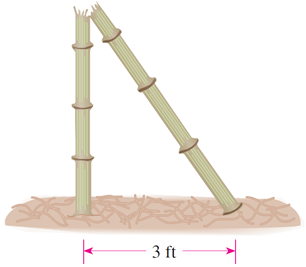
\includegraphics{bamboo.png}
\caption{Diagram from Problem 3}
\end{figure} 

\textbf{Solution:}

Let the base of the bamboo be A, the break point be B, and the tip of the bamboo be C.\\
Since $AB + BC = 10$, $AB = 10 - BC$.
\begin{align*}
    BC^2 &= AB^2 + AC^2\\
    BC^2 &= (10 - BC)^2 + 3^2\\
    BC^2 &= 100 - 20BC + BC^2 + 9\\
    0 &= 100 - 20BC + BC^2 + 9 - BC^2\\
    0 &= 109 - 20BC\\
    BC &= \dfrac{-109}{-20}\\
    BC &= 5.45 ft
\end{align*}
$AB = 10 - 5.45$\\
$AB = 4.55 ft$\\

\textbf{Therefore, the height of the break is 4.55 feet.}

\newpage

%% PROBLEM 4
\item A wire 100cm in length is cut in to two pieces. One piece is formed into a circle and the other into an equilateral triangle. If the two figures have the same area, determine the lengths of the two pieces of wire.\\
%%===================  start drawing  ===================
\begin{tikzpicture}
%    ===================  lines  ========================
%% triangle
\draw (0,0) -- (60:3) -- (3,0) -- cycle;
\draw [dashed] (1.5,0) -- (1.5, 2.5);
%% circle
\draw (8,1.5) circle (1.5cm);
\draw [red] (8,1.5) -- (9.5, 1.5);
%%=======================================================
%   =========  C++ equivalent of initializing  ==========
\coordinate (r) (8.2,1.5);
\coordinate (h) (1.5, 0.5);
\coordinate (d) (2.6, 1);
%   ================  labelling points  =================
\draw (r) (8.2, 1.5) node[above]{$r$};
\draw (h) (1.5, 1) node[right]{$h$};
\draw (d) (2.6, 1) node[above]{$d$};
\end{tikzpicture}\\
%%===================  end drawing  =====================

\textbf{Solution:}

Let $r$ be the radius of the circle.\\
Let $d$ be one side length of the equilateral triangle and $h$ be the height of the triangle.\\
Based on the given information, we have the following:
\begin{align*}
    2\pi r + 3d &=  100\\
    \pi r^2 &=  S_{triangle}
\end{align*}


\textbf{Determine the area of the equilateral triangle}\\
\textit{Determining the height}
%% Note: \left outside, \right inside
\setcounter{equation}{0} %% resets line numbers
\begin{align}
    h^2 &= d^2 - \left(\dfrac{d}{2}\right)^2\\
    h^2 &= d^2 - \dfrac{d^2}{4}\\
    h^2 &= \dfrac{4d^2-d^2}{4}\\
    h^2 &= \dfrac{3d^2}{4}\\
    h &= \sqrt{\dfrac{3d^2}{4}}\\
    h &= \dfrac{d\sqrt{3}}{2}
\end{align}
\textit{Determining the area}\\
Since the $S_{triangle} = \dfrac{l \times h}{2}$, $l = d$ and $h = \dfrac{d\sqrt{3}}{2}$, we have:
\setcounter{equation}{0}
\begin{align}
    S_{triangle} &= \dfrac{d \times \dfrac{d\sqrt{3}}{2}}{2}\\
    S_{triangle} &= \dfrac{d \times d\sqrt{3}}{4}\\
    S_{triangle} &= \dfrac{d^2 \times \sqrt{3}}{4}
\end{align}\\

Now that we have the area of the equilateral triangle, we can sub in $\dfrac{d^2 \times \sqrt{3}}{4}$ into $S_{triangle}$ from the two equations at the beginning of the solution:
\begin{align*}
    2\pi r + 3d &=  100\\
    \pi r^2 &=  \dfrac{d^2 \times \sqrt{3}}{4}
\end{align*}
\textbf{Determine side length d}\\
Rearranging the first equation will remove $r$ leaving us with only one variable to solve, $d$.\\
\begin{align*}
    2\pi r + 3d &=  100\\
    r &= \dfrac{100 - 3d}{2\pi}
\end{align*}
Sub in $\dfrac{100 - 3d}{2\pi} = r$. Determine side length, $d$, of the equilateral triangle.
\begin{align*}
    \pi r^2 &=  \dfrac{d^2 \times \sqrt{3}}{4}\\
    \pi \left(\dfrac{100 - 3d}{2\pi} \right)^2 &= \dfrac{d^2 \times \sqrt{3}}{4}\\
    \dfrac{100^2 - 600d + 9d^2}{4\pi^2} &= \dfrac{d^2\sqrt{3}}{4\pi}\\
    \dfrac{100^2 - 600d + 9d^2}{4\pi^2} \times 4 \pi &= \dfrac{d^2\sqrt{3}}{4\pi} \times 4 \pi\\
    \dfrac{100^2 - 600d + 9d^2}{\pi} &= d^2\sqrt{3}\\
    100^2 - 600d + 9d^2 &= \pi d^2\sqrt{3}\\
    0 &=  100^2 - 600d + 9d^2 -  \pi d^2\sqrt{3}\\
    0 &=  9d^2 -  \pi d^2\sqrt{3} - 600d + 10000\\
    0 &=  (9 - \pi \sqrt{3})d^2 - 600d + 10000
\end{align*}
The equation is now in the standard quadratic form. We can now determine $d$ by using the quadratic formula, $x = \dfrac{-b  \pm \sqrt{b^2 - 4ac}}{2a}$.\\
\begin{align*}
    x_1 &= \dfrac{-(-600) + \sqrt{(-600)^2 - 4(9 - \pi \sqrt{3})(10000)}}{2(9 - \pi \sqrt{3})}\\
    x_1 &\approx 149.85324549493623 \text{ cm}\\
    x_2 &= \dfrac{600 - \sqrt{(-600)^2 - 4(9 - \pi \sqrt{3})(10000)}}{2(9 - \pi \sqrt{3})}\\
    x_2 &\approx 18.752295565776265 \text{ cm}
\end{align*}
Since the wire is only 100 cm long, only $x_2$ is a valid answer as $x_1 > 100$. Therefore, $d \approx 18.753$ cm.\\
$d$ is only the measurement of 1 side length of the equilateral triangle, therefore the perimeter or length of wire of the triangle $= 3d$.\\

\textbf{Determine the length of each piece of wire}\\
Let $a$ be the length of wire for the triangle and $b$ be the length of wire for the circle.
\begin{align*}
    a &= 3d\\
    a &= 3(18.752295565776265)\\
    a &\approx 56.2568865 \text{ cm}\\
    &\hrulefill\\
    b &= 100 - a\\
    b &= 100 - 56.2568865\\
    b &\approx 43.7431135 \text{ cm}
\end{align*}
\textbf{Therefore, the length of wire for the triangle is roughly 56.26 cm and the length of wire for the circle is roughly 43.74 cm.}
\newpage

%% PROBLEM 5
\item Prove or disprove that the sum of any two increasing functions is increasing.\\

\textbf{Solution:}

An increasing function is a function where the y-value increases as the x-value increases. Consider two increasing functions $f(x)$ and $g(x)$ where in both functions, $x_2 > x_1$. Since $x_2 > x_1$ and they are both increasing functions, $f(x_2) > f(x_1)$ and $g(x_2) > g(x_1)$ because as x increases, the output also increases.\\

Let $h(x)$ be the sum of $f(x)$ and $g(x)$ and take a look at the following statement:\\

$h(x) = f(x) + g(x)$\\
$h(x_1) = f(x_1) + g(x_1)$\\
$h(x_2) = f(x_2) + g(x_2)$\\

For the sum $h(x)$ to be an increasing function, $h(x)$ must increase as $x$ increases, therefore, $h(x_2)$ must be larger than $h(x_1)$. Consider the following:
\setcounter{equation}{0}
\begin{align*}
    &f(x_2) > f(x_1)\MoveEqLeft[1]\\
    \times &\hspace{0.1cm} g(x_2) > g(x_1)\\
    &\noindent\rule{6cm}{0.4pt}\\
    &f(x_2) + g(x_2) > f(x_1) + g(x_1)
\end{align*}\\
Since $h(x_1) = f(x_1) + g(x_1)$ and $h(x_2) = f(x_2) + g(x_2)$, the inequality $f(x_2) + g(x_2) > f(x_1) + g(x_1)$ also means that $h(x_2) > h(x_1)$. And since the larger x-value results in a larger y-value, $h(x)$ is an increasing function.\\

\textbf{Therefore, the sum of any two increasing functions is increasing.}

\newpage

%% PROBLEM 6
\item Prove or disprove that the product of any two increasing functions is increasing.\\

\textbf{Solution: }

I will disprove this statement by counterexample. By definition, an increasing function is a function where the y-value increases as the x-value increases. So, consider two increasing functions, $f(x)$ and $g(x)$ where $f(x) = x + 1$ and $g(x) = x - 1$. Determine the product of these two functions to see if the result is an increasing function or not.
\begin{align*}
    f(x) \times g(x) &= (x+1)(x-1)\\
    h(x) &= x^2 - x + x -1\\
    h(x) &= x^2 - 1
\end{align*}
We can see that h(x) is no longer an increasing function because it is a quadratic function. In this specific function of $h(x)$, it has a behaviour where as the x-value increases from $-\infty$ to 0, the y-value is decreasing.\\

\textbf{Therefore, increasing functions are not closed under multiplication.}


\newpage

%% PROBLEM 7
\item Prove that the only solution to $3^x + 4^x = 5^x$ is $x=2$.\\

\textbf{Solution:}

\begin{figure}[h]
\centering
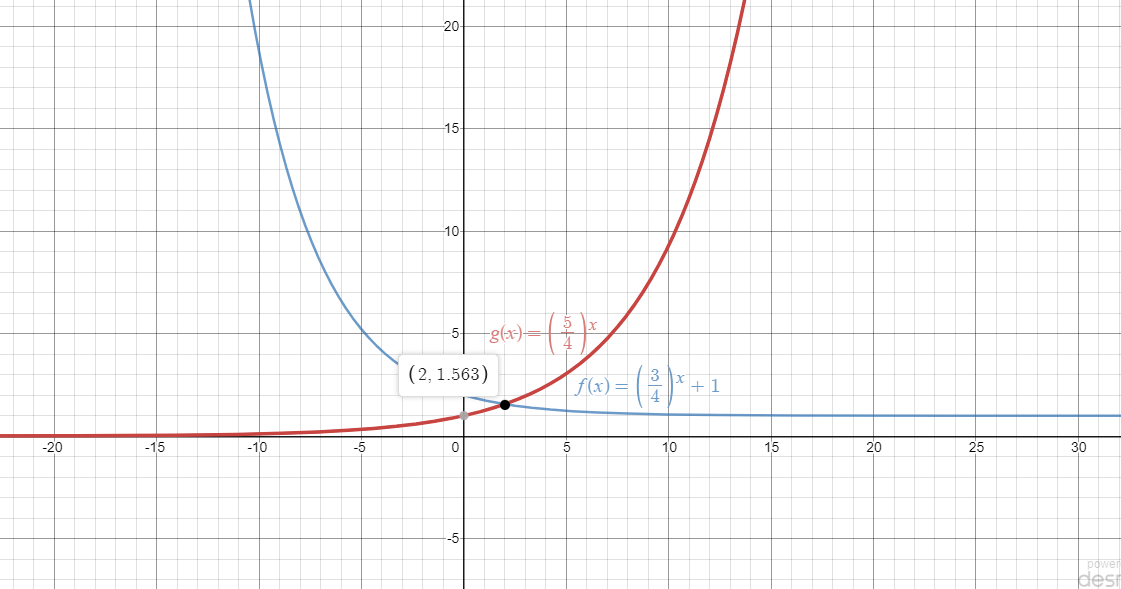
\includegraphics[width=1\textwidth]{Q7Graph.png}
\caption{Graph of g(x) and f(x)}
\end{figure} 

Manipulate the equation to remove the term $4^x$.
\setcounter{equation}{0}
\begin{align}
    3^x + 4^x &= 5^x\\
    \dfrac{3^x+4^x}{4^x} &= \dfrac{5^x}{4^x}\\
    \dfrac{3^x}{4^x} + 1 &= \dfrac{5^x}{4^x}\\
    \left(\dfrac{3}{4} \right)^x + 1 &= \left(\dfrac{5}{4} \right)^x
\end{align}\\
Now that $4^x$ is removed from the equation, we have the new equation $\left(\dfrac{3}{4} \right)^x + 1 = \left(\dfrac{5}{4} \right)^x$\\

Separate the left and the right side of the equation to make two functions. We have $f(x) = \left(\dfrac{3}{4} \right)^x + 1$, highlighted in blue, and $g(x) = \left(\dfrac{5}{4} \right)^x$, highlighted in red.\\\\

\newpage

\textbf{Analysis of the graph to prove x can only be 2}\\

Take a look at $\left(\dfrac{3}{4} \right)^x + 1$ on line (4). As $x$ increases, the entire function decreases because the numerator has a base of 3 which is smaller compared to the denominator's base of 4. It is also translated 1 up.

As for $\left(\dfrac{5}{4} \right)^x$, as $x$ increases, the function increases because the numerator $>$ denominator.\\

We already know that one of the solutions for both sides of the equation to equal is $x = 2$. So if $x$ continues to increase, the two sides will never equal or meet on the graph because they split and get further and further away (one increases, one decreases. Logically, they will never meet).\\

The same can be said if $x < 2$. this time, the function $\left(\dfrac{5}{4}\right)^x$, which was increasing before, now decreases and $\left(\dfrac{3}{4}\right)^x$ increases as $x$ decreases. Again, they will never meet on the graph.\\\\

\textbf{Therefore, the only value of $x$ where $3^x + 4^x = 5^x$ is $x = 2$}.\\



\newpage

%% PROBLEM 8
\item Define (rewrite) $f(x) = |x^3 - x|$ as a piecewise function not including any expressions involving absolute value.\\

\textbf{Solution:}\\
\textit{**Note: For this solution, assume that I do not have Desmos and that I am only using Desmos as a tool to show a sketch of the graph $f(x)$.}\\

Firstly, sketch out $f(x)$ \textbf{without the absolute operation} to visualize the graph. We'll call this graph $g(x)$.

\begin{figure}[h]
\centering
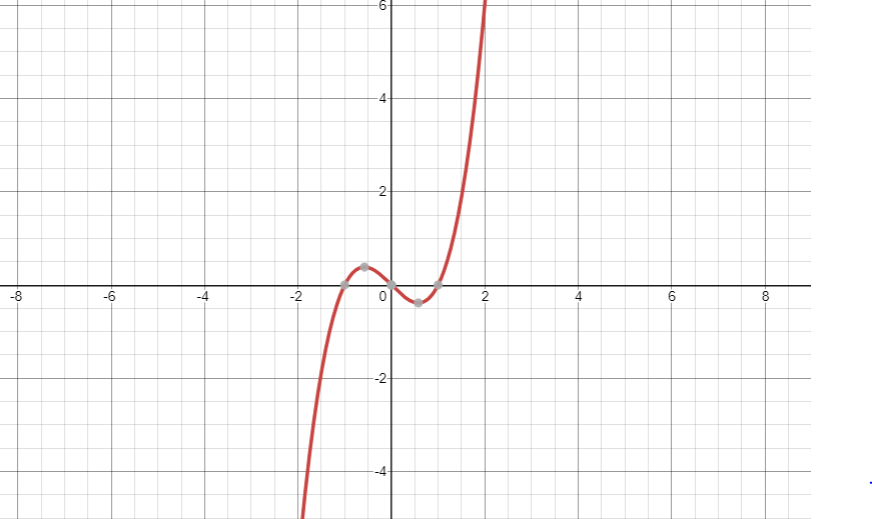
\includegraphics[width=1\textwidth]{Q8Graph.png}
\caption{Graph of $g(x) = x^3 - x$}
\end{figure}

Since an absolute function only outputs positive values including zero, all values of $x$ where the corresponding output, $f(x)$, has a value that is less than zero must be reflected on the x-axis in order to make it a positive. Looking at the sketch of the function $g(x)$, we can see two intervals that have y-values less than zero. Determine the range of those intervals by finding the zeros of $g(x)$.
\setcounter{equation}{0}
\begin{align}
    0 &= x^3 - x\\
    0 &= x(x^2 - 1)\\
    0 &= x(x-1)(x+1)
\end{align}

\begin{minipage}{.5\textwidth}
    \textbf{Therefore, the zeros are -1, 0, and 1}\\
    \end{minipage}
    \begin{minipage}{.5\textwidth}
    \begin{figure}[H]
    \centering
    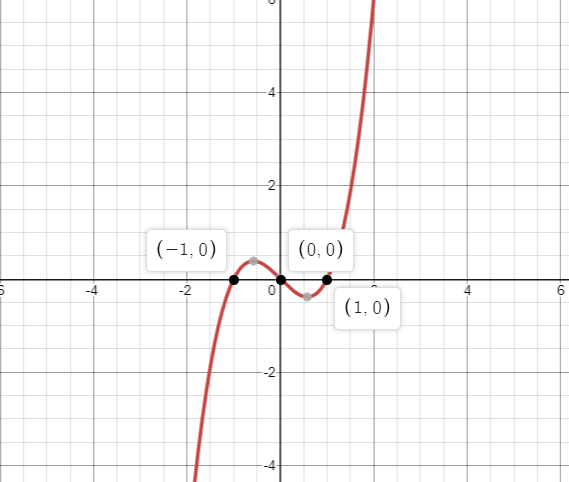
\includegraphics[width=1\textwidth]{Q8GraphLABEL.png}
    \caption{Graph of g(x) with zeros labelled}
    \end{figure}
\end{minipage}\\\\

Since $f(x)$ cannot be less than 0 as $f(x)$ is an absolute function, we can see that $g(x) = x^3 - x$ must also only include positive outputs and that all negative outputs must be reflected on the x-axis.\\

Looking at figure 4, we can see that for values of $x$ where $-1 \leq x \leq 0$ and $x \geq 1$, the function $x^3 - x$ is valid. Therefore if $x$ where $-1 \leq x \leq 0$ or $x \geq 1$, $g(x) = x^3 - x$.\\

We can also see that if $x < -1$ or $0 < x < 1$, $x^3 - x$, the function is no longer valid. In order for the invalid case to be valid, $g(x)$ must be reflected on the x-axis to make all the outputs larger or equal to zero. That means if $x < -1$ or $0 < x < 1$, $g(x) = -(x^3 - x)$. However, since the absolute function does not affect the zeros, $x = -1, 0, 1$ are valid in this this function. Therefore, if $x \leq -1$ or $0 \leq x \leq 1$, $g(x) = -(x^3 - x)$.\\

\textbf{Therefore, the function $f(x) = |x^3-x|$ written as a piecewise function is}
$$g(x) =
\begin{cases}
    x^3 - x & \text{if} \{-1 \leq x \leq 0, x \geq 1\} \\
    -(x^3 - x) & \text{if} \{0 \leq x \leq 1, x \leq -1\}
\end{cases}$$

\newpage

\end{enumerate}
\end{document} 
